\section{Diseño Arquitectónico}%
\label{sec:diseno-arquitectonico}

\begin{figure}[H] % Opciones de posicionamiento: here, top, bottom, page
    \centering
    \adjustbox{max width=\textwidth, max height=\textheight}{%
        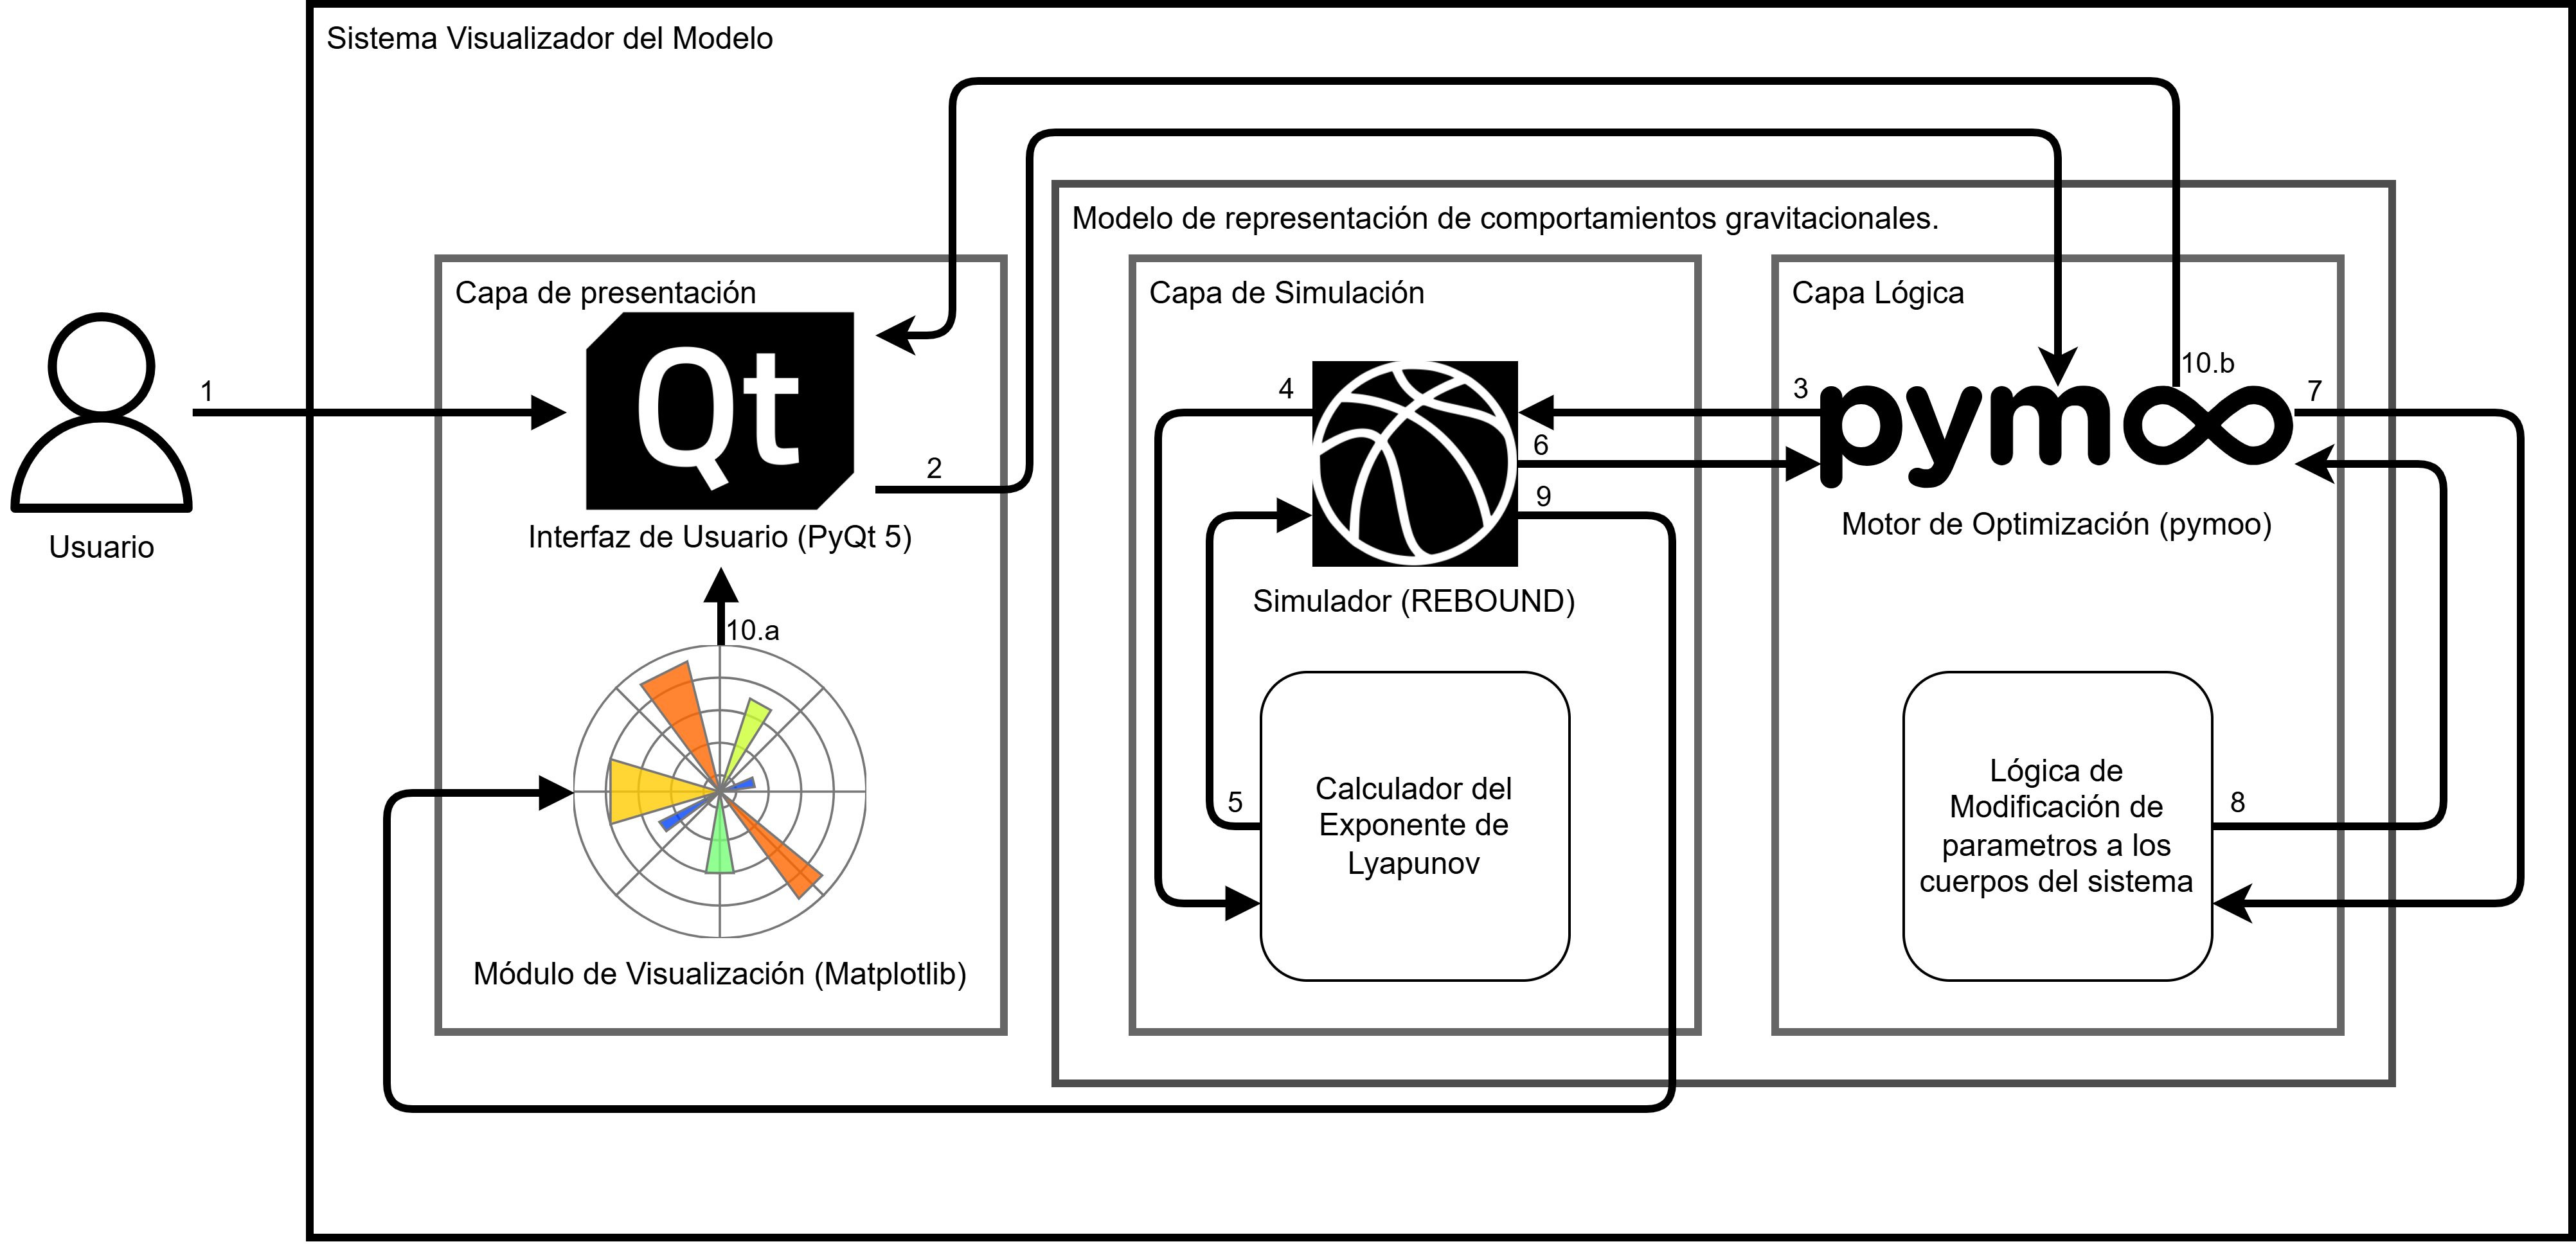
\includegraphics{img/Diseño/Arquitectura.png}
    }
    \caption{Diagrama de Arquitectura.}%
    \label{fig:architecture_diagram} % Etiqueta para referenciar la figura
\end{figure}

\subsection{Introducción y Objetivos de Diseño}

El presente diseño arquitectónico describe la estructura y organización del ``Sistema Visualizador del Modelo'', concebido para la simulación, optimización y análisis de comportamientos gravitacionales, con un enfoque inicial en sistemas de dos cuerpos. La arquitectura se fundamenta en principios de \textbf{modularidad, encapsulamiento y separación de incumbencias}, con el fin de garantizar la extensibilidad, mantenibilidad y robustez del sistema. Se ha adoptado un paradigma arquitectónico híbrido que combina un enfoque basado en componentes, una estructuración en capas lógicas y una comunicación parcialmente dirigida por eventos.

Los objetivos primordiales que guían este diseño son:
\begin{enumerate}
    \item \textbf{Modularidad y Cohesión:} Facilitar el desarrollo, prueba y mantenimiento independientes de los distintos módulos funcionales.
    \item \textbf{Bajo Acoplamiento:} Minimizar las dependencias entre componentes para permitir la sustitución o mejora de tecnologías individuales (\texttt{e.g.}, motor de simulación, biblioteca de optimización) con un impacto reducido en el resto del sistema.
    \item \textbf{Capacidad de Modificación Dinámica:} Soportar la alteración de parámetros clave del sistema (\texttt{ej.} masas) durante la ejecución del ciclo de optimización.
    \item \textbf{Eficiencia Computacional:} Integrar herramientas especializadas como \texttt{REBOUND} para la simulación N-cuerpos y \texttt{pymoo} para la optimización bioinspirada, buscando un balance entre precisión y tiempo de ejecución.
    \item \textbf{Visualización Interactiva:} Proveer retroalimentación visual clara y comprensible del proceso de simulación y optimización al usuario a través de \texttt{PyQt5} y \texttt{Matplotlib}.
\end{enumerate}

La arquitectura propuesta se articula en torno a tres capas principales: Presentación, Lógica y Simulación/Datos, cada una con componentes especializados que interactúan mediante interfaces bien definidas.

\subsection{Arquitectura en Capas y Componentes Principales}

El sistema se organiza en las siguientes capas lógicas, cada una agrupando componentes con responsabilidades cohesivas:

\subsubsection{Capa de Presentación}
\textbf{Propósito General:} Gestionar toda la interacción con el usuario final, desde la captura de datos de entrada hasta la visualización de resultados y el estado del sistema. Esta capa abstrae los detalles de la interfaz gráfica y la representación de datos del resto de la lógica del sistema.

\begin{enumerate} % CAMBIADO DE itemize A enumerate
    \item \textbf{2.1.1. Interfaz de Usuario (UI)}
    \begin{itemize}
        \item \textbf{Tecnología:} \texttt{PyQt5}.
        \item \textbf{Responsabilidades Fundamentales:}
        \begin{itemize}
            \item \textbf{Recolección y Validación de Parámetros:} Presenta formularios y controles para que el usuario ingrese los parámetros iniciales de la simulación (\texttt{e.g.}, masas, posiciones, velocidades iniciales de los cuerpos) y los parámetros de configuración del algoritmo de optimización (\texttt{e.g.}, tamaño de la población, número de generaciones, criterios de parada, rangos de los parámetros a optimizar). Implementa rutinas de validación para asegurar la coherencia y admisibilidad de los datos antes de iniciar cualquier proceso.
            \item \textbf{Iniciación y Control de Procesos:} Actúa como el punto de entrada para disparar el ciclo de optimización invocando al Motor de Optimización. Permite al usuario iniciar, pausar o detener los procesos.
            \item \textbf{Presentación de Resultados y Retroalimentación:} Despliega los resultados finales de la optimización (mejor conjunto de parámetros, valor de fitness correspondiente) y provee retroalimentación en tiempo real sobre el progreso del algoritmo de optimización (\texttt{e.g.}, número de generación actual, mejor fitness de la generación).
        \end{itemize}
        \item \textbf{Datos Manejados:}
        \begin{itemize}
            \item \textit{Entrada:} Parámetros de configuración de simulación y optimización, eventos de control del usuario.
            \item \textit{Salida:} Representación textual y gráfica de resultados, estado del sistema.
        \end{itemize}
    \end{itemize}

    \item \textbf{2.1.2. Módulo de Visualización}
    \begin{itemize}
        \item \textbf{Tecnología:} \texttt{Matplotlib}, integrado en la UI de \texttt{PyQt5}.
        \item \textbf{Responsabilidades Fundamentales:}
        \begin{itemize}
            \item \textbf{Generación de Representaciones Gráficas:} Transforma los datos numéricos provenientes de la Capa de Simulación (trayectorias, estados energéticos) y de la Capa Lógica (progreso de la optimización) en visualizaciones comprensibles.
            \item \textbf{Renderizado y Actualización Dinámica:} Es responsable de renderizar los gráficos (\texttt{e.g.}, trayectorias orbitales 2D/3D, evolución de la energía del sistema, convergencia del fitness) dentro de los widgets designados en la UI./ Soporta la actualización dinámica de estos gráficos para reflejar el estado cambiante durante la simulación y la optimización.
            \item \textbf{Procesamiento de Datos para Visualización:} Realiza las transformaciones necesarias sobre los datos crudos (\texttt{e.g.}, escalado, selección de subconjuntos de datos, cálculo de métricas derivadas para visualización) para adecuarlos a los requisitos de \texttt{Matplotlib} y a las preferencias del usuario.
        \end{itemize}
        \item \textbf{Datos Manejados:}
        \begin{itemize}
            \item \textit{Entrada:} Series temporales de posiciones y velocidades, valores de energía, métricas de fitness, configuración de visualización.
            \item \textit{Salida:} Objetos gráficos de \texttt{Matplotlib} (figuras, ejes, primitivas de dibujo).
        \end{itemize}
    \end{itemize}
\end{enumerate}

\subsubsection{Capa Lógica}
\textbf{Propósito General:} Orquestar el proceso de optimización de parámetros. Contiene la inteligencia para guiar la búsqueda de soluciones óptimas y adaptar los parámetros del sistema basándose en el rendimiento observado.

\begin{enumerate} % CAMBIADO DE itemize A enumerate
    \item \textbf{2.2.1. Motor de Optimización}
    \begin{itemize}
        \item \textbf{Tecnología:} \texttt{pymoo}.
        \item \textbf{Responsabilidades Fundamentales:}
        \begin{itemize}
            \item \textbf{Gestión del Algoritmo Bioinspirado:} Implementa el ciclo de vida de un algoritmo genético (u otro paradigma bioinspirado soportado por \texttt{pymoo}). Esto incluye la inicialización de una población de soluciones candidatas (conjuntos de parámetros), la aplicación iterativa de operadores evolutivos (selección, cruzamiento, mutación) para generar nuevas poblaciones, y la gestión de criterios de parada.
            \item \textbf{Evaluación de la Función Objetivo (Fitness):} Para cada individuo (conjunto de parámetros) de la población, coordina su evaluación. Esto implica invocar a la Capa de Simulación para ejecutar una simulación con dichos parámetros y obtener las trayectorias, y luego utilizar el Calculador del Exponente de Lyapunov para obtener un valor escalar de fitness que cuantifique la ``calidad'' de esa solución.
            \item \textbf{Orquestación del Flujo de Optimización:} Controla el flujo iterativo, decidiendo cuándo generar una nueva población, cuándo evaluar, y cuándo terminar el proceso.
        \end{itemize}
        \item \textbf{Datos Manejados:}
        \begin{itemize}
            \item \textit{Entrada:} Configuración del algoritmo de optimización (desde la UI), valores de fitness (desde el Calculador LE).
            \item \textit{Salida:} Conjuntos de parámetros para evaluación (hacia la Capa de Simulación), mejor solución encontrada y métricas de progreso (hacia la UI).
        \end{itemize}
    \end{itemize}

    \item \textbf{2.2.2. Lógica de Modificación de Parámetros}
    \begin{itemize}
        \item \textbf{Responsabilidades Fundamentales:}
        \begin{itemize}
            \item \textbf{Aplicación de Variaciones Paramétricas:} Actúa como intermediario para aplicar los conjuntos de parámetros generados por el Motor de Optimización (\texttt{pymoo}) a las instancias de simulación en \texttt{REBOUND}. Asegura que los parámetros propuestos por los operadores genéticos (\texttt{e.g.}, masas, componentes de velocidad/posición inicial) se traduzcan correctamente en la configuración de cada simulación individual.
            \item \textbf{Retroalimentación y Adaptación del Proceso de Optimización (Potencial):} Aunque el flujo principal es que \texttt{pymoo} genere los parámetros, este módulo podría incorporar lógicas para adaptar dinámicamente el propio proceso de optimización. Por ejemplo, basándose en la convergencia observada o la diversidad de la población, podría ajustar hiperparámetros de \texttt{pymoo} (como tasas de mutación/cruzamiento) o refinar los rangos de búsqueda de los parámetros, interactuando para ello con el Motor de Optimización.
        \end{itemize}
        \item \textbf{Datos Manejados:}
        \begin{itemize}
            \item \textit{Entrada:} Nuevos conjuntos de parámetros (individuos) generados por \texttt{pymoo}.
            \item \textit{Salida:} Parámetros configurados para instancias específicas del Simulador \texttt{REBOUND}.
        \end{itemize}
    \end{itemize}
\end{enumerate}

\subsubsection{Capa de Simulación y Datos}
\textbf{Propósito General:} Ejecutar las simulaciones físicas y realizar los cálculos necesarios para evaluar la calidad de las configuraciones paramétricas. Esta capa encapsula la física del problema y las herramientas numéricas para su resolución.

\begin{enumerate} % CAMBIADO DE itemize A enumerate
    \item \textbf{2.3.1. Simulador}
    \begin{itemize}
        \item \textbf{Tecnología:} \texttt{REBOUND}.
        \item \textbf{Responsabilidades Fundamentales:}
        \begin{itemize}
            \item \textbf{Modelado del Sistema Físico:} Configura y ejecuta simulaciones del problema de N-cuerpos (inicialmente dos cuerpos) de acuerdo con los parámetros proporcionados (masas, posiciones iniciales, velocidades iniciales, constante gravitacional \texttt{G}, paso de tiempo \texttt{dt}, tiempo máximo de simulación \texttt{T\_max}).
            \item \textbf{Integración Numérica:} Utiliza los integradores numéricos provistos por \texttt{REBOUND} (\texttt{e.g.}, WHFast, IAS15) para avanzar el estado del sistema en el tiempo, calculando las trayectorias de los cuerpos bajo la influencia de sus interacciones gravitacionales mutuas.
            \item \textbf{Provisión de Datos de Trayectoria:} Exporta los resultados de la simulación, típicamente como series temporales de las posiciones y velocidades de cada cuerpo, que son consumidos por el Calculador del Exponente de Lyapunov y, opcionalmente, por el Módulo de Visualización.
        \end{itemize}
        \item \textbf{Datos Manejados:}
        \begin{itemize}
            \item \textit{Entrada:} Parámetros físicos y de simulación (masas, estado inicial, \texttt{G}, \texttt{dt}, \texttt{T\_max}, integrador a usar).
            \item \textit{Salida:} Series temporales de vectores de posición y velocidad para cada cuerpo.
        \end{itemize}
    \end{itemize}

    \item \textbf{2.3.2. Calculador del Exponente de Lyapunov (LE)}
    \begin{itemize}
        \item \textbf{Responsabilidades Fundamentales:}
        \begin{itemize}
            \item \textbf{Cuantificación de la Estabilidad Dinámica:} Implementa el algoritmo para calcular el Exponente de Lyapunov Máximo (MLE) a partir de las trayectorias generadas por el Simulador. El LE es una métrica fundamental en la teoría de sistemas dinámicos que mide la tasa promedio de separación exponencial de trayectorias inicialmente cercanas. Un LE positivo indica comportamiento caótico, mientras que un LE cercano a cero o negativo sugiere estabilidad u orbitalidad regular.
            \item \textbf{Función de Fitness:} Provee el valor del LE calculado como la función objetivo (o un componente principal de ella) al Motor de Optimización. El objetivo de la optimización es, típicamente, encontrar conjuntos de parámetros que minimicen el LE, buscando configuraciones de mayor estabilidad.
            \item \textbf{Procesamiento de Trayectorias:} Toma como entrada los datos de trayectoria (series temporales de estado) de dos o más simulaciones ligeramente perturbadas (o utiliza métodos basados en la evolución de vectores tangentes) para estimar la tasa de divergencia.
        \end{itemize}
        \item \textbf{Datos Manejados:}
        \begin{itemize}
            \item \textit{Entrada:} Datos de trayectoria (posiciones, velocidades a lo largo del tiempo) de \texttt{REBOUND}.
            \item \textit{Salida:} Un valor escalar representando el Exponente de Lyapunov.
        \end{itemize}
    \end{itemize}
\end{enumerate}

\subsection{Interacciones Principales y Flujos de Datos y Control}

El funcionamiento coordinado del sistema se basa en una serie de interacciones clave entre sus componentes. A continuación, se detallan estos flujos de control y datos, numerados según la descripción original y expandidos para mayor claridad:

\begin{enumerate}
    \item \textbf{Usuario $\rightarrow$ Interfaz de Usuario (Inicio y Configuración Inicial):}
    \begin{itemize}
        \item \textbf{Disparador:} Acción del operador humano.
        \item \textbf{Acción:} El usuario interactúa con la Interfaz de Usuario (UI) para introducir los parámetros fundamentales de la simulación (\texttt{e.g.}, valores nominales o rangos para las masas de los dos cuerpos, sus posiciones y velocidades iniciales), la constante gravitacional \texttt{G}, el paso de tiempo \texttt{dt} para la integración numérica, y el tiempo máximo de simulación \texttt{T\_max} para cada evaluación individual. Adicionalmente, se configuran los parámetros del Motor de Optimización (\texttt{pymoo}), tales como el tamaño de la población de soluciones, el número máximo de generaciones, los criterios de parada, y la especificación de qué parámetros físicos (\texttt{e.g.}, masas) serán optimizados junto con sus rangos de búsqueda permitidos. La activación de un control en la UI (\texttt{e.g.}, botón ``Iniciar Simulación/Optimización'') formaliza la entrada de estos datos.
        \item \textbf{Datos Intercambiados:} Estructuras de datos o variables conteniendo los valores numéricos y selecciones de configuración ingresados por el usuario.
        \item \textbf{Resultado Esperado:} La UI valida internamente la coherencia y admisibilidad de los parámetros (\texttt{e.g.}, rangos lógicos, tipos de datos correctos) y los prepara para su posterior procesamiento y distribución a las capas correspondientes.
    \end{itemize}

    \item \textbf{Interfaz de Usuario $\rightarrow$ Capa de Simulación (Configuración de Simulación Base/Visualización Directa~-~\textit{Contexto Específico}):}
    \begin{itemize}
        \item \textbf{Disparador:} Podría ser una acción del usuario para una simulación directa sin optimización, o un paso de configuración previo a la optimización.
        \item \textbf{Acción:} En un escenario donde el usuario desee ejecutar una simulación única con parámetros fijos (sin pasar por el ciclo de optimización bioinspirada) o para establecer una simulación base, la UI enviaría los parámetros validados (masas, posiciones, \texttt{dt}, \texttt{G}, \texttt{T\_max}) directamente al subsistema de simulación (específicamente al Simulador \texttt{REBOUND} a través de una lógica de control simplificada).
        \item \textbf{Datos Intercambiados:} Conjunto completo de parámetros físicos y de simulación necesarios para una ejecución de \texttt{REBOUND}.
        \item \textbf{Resultado Esperado:} El Simulador \texttt{REBOUND} se configura y está listo para ejecutar una integración numérica.\ \textit{Nota: En el flujo principal de optimización, esta interacción directa es menos prominente, ya que el Motor de Optimización gestiona las invocaciones a \texttt{REBOUND}.}
    \end{itemize}

    \item \textbf{Interfaz de Usuario $\rightarrow$ Motor de Optimización (\texttt{pymoo}) (Inicio del Ciclo Evolutivo):}
    \begin{itemize}
        \item \textbf{Disparador:} Evento de ``inicio'' generado por la UI tras la validación de los parámetros de configuración (como se describe en la Interacción 1), específicamente cuando el objetivo es la optimización.
        \item \textbf{Acción:} La UI transfiere la configuración completa del problema de optimización al Motor de Optimización (\texttt{pymoo}). Esto incluye la definición de las variables de diseño (qué parámetros físicos se optimizan), sus límites (rangos de búsqueda), la función objetivo (implícitamente, minimizar el LE), y los parámetros del algoritmo genético (tamaño de población, número de generaciones, etc.).
        \item \textbf{Datos Intercambiados:} Objeto o estructura de datos que encapsula la definición del problema de optimización y los hiperparámetros del algoritmo genético.
        \item \textbf{Resultado Esperado:} \texttt{pymoo} se inicializa, creando la primera población de individuos (conjuntos de parámetros candidatos) de acuerdo con la estrategia de inicialización configurada (\texttt{e.g.}, muestreo aleatorio dentro de los rangos).
    \end{itemize}

    \item \textbf{Motor de Optimización (\texttt{pymoo}) $\rightarrow$ Simulador (\texttt{REBOUND}) (Solicitud de Evaluación de Individuo):}
    \begin{itemize}
        \item \textbf{Disparador:} Necesidad del Motor de Optimización de evaluar el fitness de cada individuo (conjunto de parámetros) en la población actual.
        \item \textbf{Acción:} Para cada individuo, \texttt{pymoo} instruye (a través de la Lógica de Modificación de Parámetros si actúa como intermediaria, o directamente) al Simulador \texttt{REBOUND} para que ejecute una simulación. Los parámetros específicos del individuo (\texttt{e.g.}, masas \texttt{m1}, \texttt{m2} propuestas por \texttt{pymoo}) se utilizan para configurar esta instancia particular de la simulación, junto con los parámetros de simulación globales (\texttt{G}, \texttt{dt}, \texttt{T\_max}).
        \item \textbf{Datos Intercambiados:} Vector de parámetros del individuo actual y parámetros de simulación fijos.
        \item \textbf{Resultado Esperado:} El Simulador \texttt{REBOUND} ejecuta una integración numérica completa para el conjunto de parámetros dado, generando una trayectoria.
    \end{itemize}

    \item \textbf{Simulador (\texttt{REBOUND}) $\rightarrow$ Calculador del Exponente de Lyapunov (Provisión de Trayectorias):}
    \begin{itemize}
        \item \textbf{Disparador:} Conclusión exitosa de una simulación en \texttt{REBOUND} para un individuo específico.
        \item \textbf{Acción:} \texttt{REBOUND} hace disponibles los datos de la trayectoria resultante. Esto típicamente comprende una serie temporal de los vectores de estado (posiciones y velocidades) de los dos cuerpos a lo largo del tiempo de simulación \texttt{T\_max}.
        \item \textbf{Datos Intercambiados:} Estructura de datos (\texttt{e.g.}, array multidimensional, lista de tuplas) que representa la evolución temporal del sistema.
        \item \textbf{Resultado Esperado:} El Calculador LE recibe estos datos y está preparado para realizar el cómputo del Exponente de Lyapunov.
    \end{itemize}

    \item \textbf{Motor de Optimización (\texttt{pymoo}) $\rightarrow$ Simulador (\texttt{REBOUND}) (Invocaciones Múltiples para Evaluación):}
    \begin{itemize}
        \item \textbf{Clarificación:} Esta interacción es una generalización de la Interacción 4. No es una interacción separada en el flujo secuencial, sino que enfatiza que el Motor de Optimización (\texttt{pymoo}) realizará múltiples solicitudes de simulación a \texttt{REBOUND}, una por cada individuo en la población actual que necesita ser evaluado, y esto se repetirá para cada nueva generación de individuos cuyos parámetros han sido ``mutados'' (modificados por operadores genéticos como cruzamiento y mutación).
        \item \textbf{Acción y Resultado:} Idénticos a la Interacción 4, pero repetidos para cada individuo de la población que \texttt{pymoo} necesita evaluar en una generación dada.
    \end{itemize}

    \item \textbf{Motor de Optimización (\texttt{pymoo}) $\rightarrow$ Interfaz de Usuario (Retroalimentación de Progreso y Resultados):}
    \begin{itemize}
        \item \textbf{Disparador:} Típicamente al final de cada generación del algoritmo evolutivo, o al alcanzar un criterio de parada.
        \item \textbf{Acción:} \texttt{pymoo} comunica al UI el estado actual del proceso de optimización. Esto incluye métricas como el número de la generación actual, el mejor valor de fitness (LE mínimo) encontrado en esa generación o hasta el momento, y opcionalmente, los parámetros del individuo que logró dicho mejor fitness. Si el proceso ha concluido, se envían los resultados finales.
        \item \textbf{Datos Intercambiados:} Valores numéricos de métricas de optimización, y potencialmente el vector de parámetros del mejor individuo.
        \item \textbf{Resultado Esperado:} La UI actualiza sus elementos visuales (\texttt{e.g.}, campos de texto, barras de progreso, gráficos de convergencia) para informar al usuario sobre el avance y los resultados de la optimización.
    \end{itemize}

    \item \textbf{Lógica de Modificación de Parámetros $\rightarrow$ Motor de Optimización (\texttt{pymoo}) (Adaptación Dinámica del Proceso de Optimización):}
    \begin{itemize}
        \item \textbf{Disparador:} Podría ser activado por hitos en el proceso de optimización (\texttt{e.g.}, después de un cierto número de generaciones, o si se detecta estancamiento en la convergencia del fitness).
        \item \textbf{Acción:} La Lógica de Modificación de Parámetros, basándose en el análisis del progreso de la optimización (\texttt{e.g.}, diversidad de la población, tasa de mejora del fitness), podría proponer ajustes a los hiperparámetros del Motor de Optimización (\texttt{pymoo}). Esto podría incluir la modificación dinámica de los rangos de búsqueda para ciertos parámetros físicos (si se observa que las mejores soluciones se concentran en subregiones) o el ajuste de las tasas de los operadores genéticos (\texttt{e.g.}, aumentar la mutación si la diversidad es baja).
        \item \textbf{Datos Intercambiados:} Nuevos valores para hiperparámetros de \texttt{pymoo} o nuevos límites para las variables de diseño.
        \item \textbf{Resultado Esperado:} \texttt{pymoo} incorpora estos ajustes en las subsiguientes generaciones, potencialmente mejorando la eficiencia o la capacidad de exploración del algoritmo de optimización.
    \end{itemize}

    \item \textbf{Simulador (\texttt{REBOUND}) $\rightarrow$ Motor de Optimización (\texttt{pymoo}) (Provisión de Datos Adicionales para Análisis):}
    \begin{itemize}
        \item \textbf{Disparador:} Finalización de una simulación en \texttt{REBOUND}, concurrente con la Interacción 5.
        \item \textbf{Acción:} Además de las trayectorias completas necesarias para el cálculo del LE, \texttt{REBOUND} podría reenviar al Motor de Optimización (posiblemente a través de la Lógica de Modificación de Parámetros) datos intermedios o estados finales específicos (\texttt{e.g.}, energía total final del sistema, momento angular, distancia mínima entre cuerpos durante la simulación).
        \item \textbf{Datos Intercambiados:} Valores escalares o vectores representando métricas adicionales de la simulación.
        \item \textbf{Resultado Esperado:} \texttt{pymoo} o la Lógica de Modificación de Parámetros pueden utilizar estos datos para análisis de convergencia más sofisticados, para la implementación de restricciones en el problema de optimización (\texttt{e.g.}, penalizar soluciones que no conservan la energía), o para refinar la función de fitness más allá del simple LE.\
    \end{itemize}

    \item \textbf{Visualización y Actualizaciones de UI:}
    \begin{itemize}
        \item \textbf{(a) Módulo de Visualización $\rightarrow$ Interfaz de Usuario (Renderizado de Gráficos):}
            \begin{itemize}
                \item \textbf{Disparador:} Solicitud de la UI para visualizar una trayectoria específica (\texttt{e.g.}, la del mejor individuo de la generación actual) o datos de simulación.
                \item \textbf{Acción:} El Módulo de Visualización, utilizando \texttt{Matplotlib}, procesa los datos de trayectoria o estado recibidos (que originalmente provinieron de \texttt{REBOUND} y fueron gestionados por la UI o el Motor de Optimización) y genera las representaciones gráficas correspondientes (\texttt{e.g.}, órbitas, gráficos de energía vs.\ tiempo).\ Estos gráficos se renderizan o actualizan dentro de los widgets designados en la UI.\
                \item \textbf{Datos Intercambiados:} Objetos gráficos de \texttt{Matplotlib}.
                \item \textbf{Resultado Esperado:} El usuario observa una representación visual actualizada del comportamiento del sistema o del progreso de la optimización.
            \end{itemize}
        \item \textbf{(b) Motor de Optimización $\rightarrow$ UI / Indicadores (Actualización de Estado en Tiempo Real):}
            \begin{itemize}
                \item \textbf{Disparador:} Emisión de eventos de estado por parte de \texttt{pymoo} (como se mencionó en la Interacción 7).
                \item \textbf{Acción:} La UI recibe estos eventos o datos de estado (\texttt{e.g.}, número de generación, mejor fitness actual) y actualiza los componentes visuales correspondientes, como barras de progreso, etiquetas de texto o gráficos de convergencia de fitness.
                \item \textbf{Datos Intercambiados:} Métricas de estado de la optimización.
                \item \textbf{Resultado Esperado:} El usuario obtiene una retroalimentación continua y en tiempo (casi) real sobre el estado del proceso de optimización.
            \end{itemize}
    \end{itemize}
\end{enumerate}

\subsection{Estilo y Paradigmas Arquitectónicos}

La arquitectura del sistema se adhiere a los siguientes estilos y paradigmas para alcanzar los objetivos de diseño:

\begin{itemize}
    \item \textbf{Arquitectura Basada en Componentes (Component-Based Architecture):}
    \begin{itemize}
        \item \textbf{Justificación:} El sistema se descompone en módulos lógicos cohesivos (UI, Módulo de Visualización, Motor de Optimización, Lógica de Modificación de Parámetros, Simulador, Calculador LE). Cada componente encapsula una funcionalidad específica y expone interfaces bien definidas (\texttt{e.g.}, APIs programáticas, llamadas a funciones) para la interacción.
        \item \textbf{Beneficios:} Este enfoque promueve la reutilización de componentes, facilita el desarrollo paralelo y las pruebas unitarias aisladas. Por ejemplo, el Simulador \texttt{REBOUND} es un componente externo con su propia API, y el Motor de Optimización \texttt{pymoo} también opera como una biblioteca con interfaces claras. La sustitución de \texttt{pymoo} por otro motor de optimización sería factible modificando principalmente la Lógica de Modificación de Parámetros y las interacciones con la UI, siempre que el nuevo motor cumpla con un protocolo de comunicación similar para la evaluación de individuos.
    \end{itemize}

    \item \textbf{Arquitectura en Capas (Layered Architecture):}
    \begin{itemize}
        \item \textbf{Justificación:} Las capas (Presentación, Lógica, Simulación/Datos) establecen una jerarquía de abstracción y control. Las interacciones ocurren típicamente entre capas adyacentes. La Capa de Presentación interactúa con la Capa Lógica, la cual a su vez interactúa con la Capa de Simulación/Datos.
        \item \textbf{Beneficios:} Este estilo reduce el acoplamiento global del sistema. Por ejemplo, la UI (Capa de Presentación) no necesita conocer los detalles internos de la integración numérica en \texttt{REBOUND} (Capa de Simulación/Datos); solo se comunica a través de la Capa Lógica. Esto mejora la mantenibilidad, ya que los cambios dentro de una capa (\texttt{e.g.}, actualizar la biblioteca de graficación en la Capa de Presentación) tienen un impacto mínimo en otras capas, siempre que las interfaces entre capas se mantengan estables.
    \end{itemize}

    \item \textbf{Arquitectura Dirigida por Eventos (Event-Driven Architecture)~-~Parcial:}
    \begin{itemize}
        \item \textbf{Justificación:} Principalmente en la interacción entre la UI y el Motor de Optimización, y para la actualización de la visualización. La UI genera eventos (\texttt{e.g.}, ``botón Iniciar presionado'') que disparan acciones en la Capa Lógica. A su vez, el Motor de Optimización puede emitir eventos (\texttt{e.g.}, ``nueva generación completada'', ``mejor fitness actualizado'') que son capturados por la UI para actualizar la visualización de progreso.
        \item \textbf{Beneficios:} Permite un comportamiento reactivo y desacoplado, especialmente para la interfaz de usuario. Las actualizaciones de la UI pueden ocurrir asincrónicamente a medida que el proceso de optimización avanza, proporcionando una experiencia de usuario más fluida y retroalimentación en tiempo real sin bloquear el hilo principal de la UI durante cálculos intensivos.
    \end{itemize}
\end{itemize}

\subsection{Consideraciones Adicionales de Diseño}

\begin{itemize}
    \item \textbf{Mantenibilidad:} La clara separación de responsabilidades y el uso de interfaces definidas entre componentes facilitan la comprensión del código, la localización de errores y la implementación de modificaciones o nuevas funcionalidades con menor riesgo de introducir efectos secundarios no deseados.
    \item \textbf{Escalabilidad Funcional:} La arquitectura está diseñada para ser extensible. Añadir un nuevo tipo de algoritmo de optimización implicaría desarrollar un nuevo componente o adaptar el existente en la Capa Lógica que interactúe con la API de \texttt{pymoo} o una biblioteca alternativa. De manera similar, soportar un nuevo integrador numérico en \texttt{REBOUND} sería una configuración dentro de la Capa de Simulación. La escalabilidad en términos de rendimiento para problemas de $N > 2$ cuerpos es inherentemente soportada por \texttt{REBOUND} y \texttt{pymoo} (que maneja vectores de parámetros), aunque requeriría ajustes en la Lógica de Modificación de Parámetros y en la función de fitness.
    \item \textbf{Capacidad de Pruebas:} La modularidad intrínseca permite la implementación de pruebas unitarias para cada componente de forma aislada (\texttt{e.g.}, probar el Calculador LE con trayectorias predefinidas, verificar la lógica de los operadores genéticos en \texttt{pymoo} con funciones objetivo sintéticas). Las pruebas de integración se centrarían en verificar las interacciones correctas entre componentes y capas (\texttt{e.g.}, asegurar que los parámetros de la UI se transmitan correctamente al Simulador a través del Motor de Optimización).
    \item \textbf{Protocolos de Comunicación:} Las interacciones entre componentes se realizan principalmente mediante llamadas a funciones directas dentro del mismo proceso. El intercambio de datos se realiza mediante estructuras de datos definidas (\texttt{e.g.}, listas, diccionarios de Python, arrays de NumPy para trayectorias).
\end{itemize}